\documentclass{beamer}
\usepackage[utf8]{inputenc}
\usepackage[T1]{fontenc}
\usepackage[brazilian]{babel}
\usepackage{lmodern}
\usetheme{default}
\usecolortheme{beaver}
\usepackage{graphicx,xcolor}
\usepackage{amsmath}


\newtheorem{definicao}[theorem]{Definição}
\newtheorem{teorema}[theorem]{Teorema}
\newtheorem{solucao}[theorem]{Solução}
\beamertemplatenavigationsymbolsempty

\makeatletter
\def\th@mystyle{%
	\ttfamily 
	\setbeamercolor{block title example}{bg=red!30,fg=black}
	\setbeamercolor{block body example}{bg=red!10,fg=black!80}
	\def\inserttheoremblockenv{exampleblock}
}
\makeatother
\theoremstyle{mystyle}
\newtheorem{algoritmo}[theorem]{Algoritmo}

\title{Interpolação Polinomial}
\author
{
	Prof. Jonathan Esteban Arroyo Silva	
}
\institute
{
	Departamento de Ciência da Computação\\
	Universidade Federal de São João del-Rei\\
	\texttt{silva.jea@ufsj.edu.br}
}
\date{}
\logo{\includegraphics[width=0.2\linewidth]{../ufsj-logo-site}}

\begin{document}
	
\begin{frame}[plain]
    \maketitle
\end{frame}

\begin{frame}[plain]
	\frametitle{Sumário}
	\tableofcontents
\end{frame}

\section{Introdução}
\begin{frame}
	\frametitle{Introdução}
	Num teste experimental, anotamos os valores de alguma determinada quantidade do nosso interesse em determinados instantes de tempo, obtendo um gráfico de pontos discretos semelhante a:
\begin{figure}
	\centering
	\includegraphics[width=0.8\linewidth]{Figuras/grafico_01}
	\label{fig:grafico01}
\end{figure}
\end{frame}

\begin{frame}
	\frametitle{Introdução}
	\begin{itemize}
		\item Entretanto, muitas vezes é de interesse saber o valor intermediário entre os pontos obtidos, assim, a \textbf{interpolação polinomial} vem como uma ferramenta para resolver este tipo de problema
		\item Dadas as $ n + 1 $ duplas ou pontos distintos $ (x_{0}, y_{0}), (x_{1}, y_{1}),\ldots, (x_{n}, y_{n}) $, a função interpoladora $ g(x) $ é aquela que $ g(x_{0}) = y_{0}, g(x_{1}) = y_{1},\ldots, g(x_{n}) = y_{n} $, para todos os pontos dados
	\end{itemize}
\end{frame}

\begin{frame}
	\frametitle{Introdução}
	Obtendo idealmente uma função contínua e de fácil manuseio, como sugerido no gráfico a seguir:
	\begin{figure}
		\centering
		\includegraphics[width=0.8\linewidth]{Figuras/grafico_02}
		\label{fig:grafico02}
	\end{figure}	
\end{frame}

\begin{frame}
	\frametitle{Introdução}
	\begin{itemize}
		\item Nesta disciplina iremos utilizar apenas funções polinomiais para este fim
		\begin{itemize}
			\item Uma vez que polinômios são facilmente computáveis, suas derivadas e integrais são também polinômios, trazendo muitas facilidades
		\end{itemize}
		\item Além do exemplo citado anteriormente, a interpolação polinomial é usada para aproximar uma função	$ f (x) $, quando ela é de difícil manejo:
		\begin{itemize}
			\item Assim, a interpolação será usada também para calcular a integral numérica de $ f (x) $ (cenas dos próximos capítulos)
		\end{itemize}
	\end{itemize}
\end{frame}

\begin{frame}
	\frametitle{Introdução}
	Dados $ n + 1 $ pontos distintos, como comentado anteriormente, determinar um polinômio $ P_{n} (x) $ de grau no máximo $ n $ que satisfaça:
	\begin{equation*}
		P_{n}(x_{0}) = y_{0}, P_{n}(x_{1}) = y_{1},\ldots, P_{n}(x_{n}) = y_{n}
	\end{equation*}
	não é uma tarefa simples, tendo mais de uma forma de se calcular, porém com a garantia de que ele é \textbf{único}.
\end{frame}

\begin{frame}
	\frametitle{Introdução}
	Neste sentido, procuramos um polinômio da forma:
	\begin{equation*}
		P_{n}(x) = a_{0} + a_{1}x + a_{2}x^{2} +\ldots+ a_{n}x^{n} 
	\end{equation*}
	ou seja, precisamos encontrar os coeficientes que satisfaçam o seguinte \textit{sistema linear}:
	\begin{gather*}
		P_{n}(x_{0}) = a_{0} + a_{1}x_{0} + a_{2}x_{0}^{2} +\ldots+ a_{n}x_{0}^{n} = y_{0}\\
		P_{n}(x_{1}) = a_{0} + a_{1}x_{1} + a_{2}x_{1}^{2} +\ldots+ a_{n}x_{1}^{n} = y_{1}\\
		\vdots\\
		P_{n}(x_{n}) = a_{0} + a_{1}x_{n} + a_{2}x_{n}^{2} +\ldots+ a_{n}x_{n}^{n} = y_{n}\\
	\end{gather*}
\end{frame}

\begin{frame}
	\frametitle{Introdução}
	Escrevendo de forma matricial teremos:
	\begin{equation*}
		\left[
		\begin{array}{ccccc}
			1 & x_{0} & x_{0}^{2} & \cdots & x_{0}^{n} \\
			1 & x_{1} & x_{1}^{2} & \cdots & x_{1}^{n} \\
			\vdots & \vdots & & \vdots & \vdots \\
			1 & x_{n} & x_{n}^{2} & \cdots & x_{n}^{n} \\
		\end{array}
		\right] 
		\begin{bmatrix} a_{0} \\ a_{1} \\ \vdots \\ a_{n} \end{bmatrix}
		=
		\begin{bmatrix} y_{0} \\ y_{1} \\ \vdots \\ y_{n} \end{bmatrix}
	\end{equation*}
	onde a matriz dos coeficientes é chamada de \textbf{Matriz de Vandermonde}, e sabendo que o determinante de esta matriz é diferente de zero desde que os pontos $ x_{i} $ sejam distintos.
\end{frame}

\begin{frame}
	\frametitle{Caso n=1}
	Vamos focar no caso onde teremos que interpolar uma função tendo apenas dois pontos de informação: $ (x_{0}, y_{0})$ e $ (x_{1}, y_{1}) $.
	
	Ou seja procuramos uma \textit{reta} com a cara:
	\begin{equation}\label{eq0}
			P_{1}(x) = a_{0} + a_{1}x
	\end{equation}
	e
	\begin{gather}
		\label{eq1} P_{1}(x_{0}) = a_{0} + a_{1}x_{0} = y_{0} \\
		\label{eq2} P_{1}(x_{1}) = a_{0} + a_{1}x_{1} = y_{1} 
	\end{gather}
\end{frame}

\begin{frame}
	\frametitle{Caso n=1}
	Da Eq.\ref{eq1} temos que $ a_{0} = y_{0} - a_{1}x_{0}  $, \textit{lembrando que as incógnitas são} $ a_{i} $, e substituindo na Eq.\ref{eq2} teremos:	
	\begin{gather*}
		y_{0} - a_{1}x_{0} + a_{1}x_{1} = y_{1} \\
		a_{1}(x_{1} - x_{0}) = y_{1} - y_{0}\\
		a_{1} = \dfrac{y_{1} - y_{0}}{x_{1} - x_{0}}
	\end{gather*}
\end{frame}

\begin{frame}
	\frametitle{Caso n=1}
	Substituindo os valores encontrados na Eq.\ref{eq0} teremos:
	\begin{gather*}
		P_{1}(x) =  y_{0} - \dfrac{y_{1} - y_{0}}{x_{1} - x_{0}}x_{0} + \dfrac{y_{1} - y_{0}}{x_{1} - x_{0}}x\\
		P_{1}(x) =  y_{0} + \dfrac{y_{1} - y_{0}}{x_{1} - x_{0}}(x - x_{0})\\		
	\end{gather*}
	Basta avaliar $ P_{1}(x) $ em $ x = x_{0} $ e $  x = x_{1} $ para verificar que de fato este é o polinômio interpolador de $ (x_{0} , y_{0} ) $ e $ (x_{1} , y_{1} ) $.	
\end{frame}

\begin{frame}
	\frametitle{Exemplo}
	Dada a seguinte tabela:
	\begin{table}
		\centering
		\begin{tabular}{c|cccc}
			x & 1 & 1.1 & 1.2 & 1.3 \\
			\hline
			\hline
			$ \tan(x) $ & 1.5574 & 1.9648 & 2.5722 & 3.6021 
		\end{tabular}
	\end{table}
	use interpolação linear $ (n=1) $, para estimar o valor de $ \tan(1.15) $.
\end{frame}

\begin{frame}
	\frametitle{Exemplo}
	Uma vez que utilizaremos apenas dois pontos e $ x = 1.15 $ se encontra entre os valores $ 1.1 $ e $ 1.2 $, teremos que a aproximação no ponto desejado será dada pela fórmula:
	\begin{equation*}
		\tan(1.15) \approx  1.9648 + \dfrac{2.5722 - 1.9648}{ 1.2 - 1.1}(1.15 - 1.1) = 2.2685
	\end{equation*}
	Sabendo que o valor \textit{exato} para $ \tan(1.15) = 2.2345 $, podemos afirmar que a aproximação foi razoável.
\end{frame}

\begin{frame}
	\frametitle{Exemplo}
	\begin{figure}
		\centering
		\includegraphics[width=0.9\linewidth]{Figuras/grafico_03}
		\label{fig:grafico03}
	\end{figure}
\end{frame}

\begin{frame}
	\frametitle{Caso geral}
	Dados $ (x_{i} , y_{i} ) $ para $ i = 0, 1,\ldots, n$, para encontrar o	polinômio $ P_{n} (x) $, precisamos resolver o sistema de equações lineares:
	\begin{equation*}
		\left[
		\begin{array}{ccccc}
			1 & x_{0} & x_{0}^{2} & \cdots & x_{0}^{n} \\
			1 & x_{1} & x_{1}^{2} & \cdots & x_{1}^{n} \\
			\vdots & \vdots & & \vdots & \vdots \\
			1 & x_{n} & x_{n}^{2} & \cdots & x_{n}^{n} \\
		\end{array}
		\right] 
		\begin{bmatrix} a_{0} \\ a_{1} \\ \vdots \\ a_{n} \end{bmatrix}
		=
		\begin{bmatrix} y_{0} \\ y_{1} \\ \vdots \\ y_{n} \end{bmatrix}
	\end{equation*}
	usando algum método que já estudamos (Eliminação Gaussiana,	Decomposição LU, etc).
	
	Entretanto, a matriz de \textbf{Vandermonde} costuma ser \alert{mal-condicionada}, levando a perda de precisão na solução.		
\end{frame}

\section{Forma de Lagrange}

\begin{frame}
	\frametitle{Forma de Lagrange - n=2 }
	Para ilustrar a ideia resolveremos um exemplo com três pontos distintos $ (x_{0}, y_{0})$, $ (x_{1}, y_{1}) $ e $ (x_{2}, y_{2}) $.
	Ou seja procuramos um \textit{polinômio} do tipo:
	\begin{equation*}
		P_{2}(x) = a_{0} + a_{1}x + a_{2}x^{2}
	\end{equation*}
	e
	\begin{equation*}
		P_{2}(x_{i}) = y_{i}, \;\; i=0,1,2
	\end{equation*}
\end{frame}

\begin{frame}
	\frametitle{Forma de Lagrange - n=2}
	Pela forma de Lagrange, procuraremos um polinômio da forma
	\begin{equation*}
		P_{2}(x) = y_{0}L_{0}(x) + y_{1}L_{1}(x) + y_{2}L_{2}(x)
	\end{equation*}
	sendo
	\begin{gather*}
		L_{0}(x) =  \dfrac{(x - x_{1})(x - x_{2})}{(x_{0} - x_{1})(x_{0} - x_{2})}\\
		L_{1}(x) =  \dfrac{(x - x_{0})(x - x_{2})}{(x_{1} - x_{0})(x_{1} - x_{2})}\\
		L_{2}(x) =  \dfrac{(x - x_{0})(x - x_{1})}{(x_{2} - x_{0})(x_{2} - x_{1})}				
	\end{gather*}
	as chamadas \textit{funções de base de Lagrange} para interpolação quadrática.
\end{frame}

\begin{frame}
	\frametitle{Forma de Lagrange - n=2}
	\begin{figure}
		\centering
		\includegraphics[width=0.9\linewidth]{Figuras/grafico_04}
		\label{fig:grafico04}
	\end{figure}
\end{frame}

\begin{frame}
	\frametitle{Forma de Lagrange - n=2}
	Essas funções possuem a seguinte propriedade:
	\begin{equation*}
		L_{i}(x_{j}) = \left\lbrace
		\begin{array}{c}
			1 \mbox{ se } i = j \\
			0 \mbox{ se } i\neq j
		\end{array}
		 \right. 
	\end{equation*}
	para $ i, j = 0, 1, 2 $ sendo todas de grau 2, e consequentemente, fazendo com que $ P_{2}(x) $ tenha grau $ \leq 2 $.
	\pause
	
	Verifique se $ P_{2}(x) = y_{0}L_{0}(x) + y_{1}L_{1}(x) + y_{2}L_{2}(x)  $ respeita a condição de que $ P_{2}(x_{i}) = y_{i}, \; i=0,1,2 $.
\end{frame}

\begin{frame}
	\frametitle{Exemplo}
	Dada a seguinte tabela:
	\begin{table}
		\centering
		\begin{tabular}{c|ccc}
			x & -1 & 0 & 1  \\
			\hline
			\hline
			$ f(x) $ & 0.54 & 1 & 0.54
		\end{tabular}
	\end{table}
	teremos
	\begin{align*}
		L_{0}(x) &=  \dfrac{(x - x_{1})(x - x_{2})}{(x_{0} - x_{1})(x_{0} - x_{2})} = \dfrac{(x - 0)(x - 1)}{(-1 - 0)(-1 - 1)} = \dfrac{x(x - 1)}{2}\\
		L_{1}(x) &=  \dfrac{(x - x_{0})(x - x_{2})}{(x_{1} - x_{0})(x_{1} - x_{2})} = \dfrac{(x + 1)(x - 1)}{(0 + 1)(0 - 1)} = 1 - x^{2}\\
		L_{2}(x) &=  \dfrac{(x - x_{0})(x - x_{1})}{(x_{2} - x_{0})(x_{2} - x_{1})} =  \dfrac{(x + 1)(x - 0)}{(1 + 1)(1 - 0)} =  \dfrac{x(x + 1)}{2}
	\end{align*}
\end{frame}

\begin{frame}
	\frametitle{Exemplo}
	Em seguida, 
	\begin{align*}
			P_{2}(x) &= y_{0}L_{0}(x) + y_{1}L_{1}(x) + y_{2}L_{2}(x)\\
			&= (0.54)\dfrac{x(x - 1)}{2} + (1)(1 - x^{2}) + (0.54)\dfrac{x(x + 1)}{2}\\
			&= 1 - 0.46x^{2}
	\end{align*}
\end{frame}

\begin{frame}
	\frametitle{Caso geral}
	Considerando $ n + 1 $ pontos, o polinômio interpolador obtido pela forma de Lagrange será dado por:
	\begin{equation*}
		P_{n}(x) = y_{0}L_{0}(x) + \ldots + y_{n}L_{n}(x) = \sum_{i=0}^{n} y_{i}L_{i}(x)
	\end{equation*}
	sendo
	\begin{align*}
		L_{i}(x) & =  \dfrac{(x - x_{0})\cdots(x - x_{i-1})(x - x_{i+1})\cdots(x - x_{n})}{(x_{i} - x_{0})\cdots(x_{i} - x_{i-1})(x_{i} - x_{i+1})\cdots(x_{i} - x_{n})}\\
		 & = \prod_{j=0,\; j\neq i}^{n}\dfrac{(x - x_{j})}{(x_{i} - x_{j})}
	\end{align*}
\end{frame}

\begin{frame}
	\frametitle{Exemplo}
	Dada a seguinte tabela:
	\begin{table}
		\centering
		\begin{tabular}{c|cccc}
			x & 1 & 1.1 & 1.2 & 1.3 \\
			\hline
			\hline
			$ \tan(x) $ & 1.5574 & 1.9648 & 2.5722 & 3.6021 
		\end{tabular}
	\end{table}
	interpole a função com um polinômio de ordem $ n = 3 $, para estimar o valor de $ \tan(1.15) $.
\end{frame}

\begin{frame}
	\frametitle{Exemplo}
	\begin{figure}
		\centering
		\includegraphics[width=0.9\linewidth]{Figuras/grafico_05}
		\label{fig:grafico05}
	\end{figure}
\end{frame}

\begin{frame}
	\frametitle{Forma de Lagrange}
	Sendo n, \textbf{x}, \textbf{y}, r, respectivamente, o número de pontos, os vetores de coordenadas dos pontos e o valor a interpolar:
	\begin{algoritmo}
		s$\leftarrow$ 0
		Para i = 1,\ldots,n, faça:\\
		\quad c$\leftarrow$ 1\\
		\quad d$\leftarrow$ 1\\
		\quad Para j = 1,\ldots,i-1, faça:\\
		\quad\quad c$\leftarrow$ c*(r - x$ _{\texttt{j}}$)\\
		\quad\quad d$\leftarrow$ d*(x$ _{\texttt{i}}$ - x$ _{\texttt{j}}$)\\
		\quad Para j = i+1,$\ldots$,n, faça:\\
		\quad\quad c$\leftarrow$ c*(r - x$ _{\texttt{j}}$)\\
		\quad\quad d$\leftarrow$ d*(x$ _{\texttt{i}}$ - x$ _{\texttt{j}}$)\\
		\quad s$\leftarrow$ s + y$ _{\texttt{i}}$*c/d
	\end{algoritmo}
\end{frame}

\section{Diferenças divididas}

\begin{frame}
	\frametitle{Diferenças divididas}
	Um conceito importante antes de se estudar a forma de Newton para se obter o polinômio interpolador, é o do operador de diferença dividida. Sendo assim, considere a função $ f(x) $ e os pontos $ x_{i} $,
	\begin{itemize}
		\item A diferença dividida de ordem \textbf{zero} é	simplesmente o valor de $ f $ no ponto $ x_{i} $, ou seja:
		\begin{equation*}
			f [x_{i}] = f (x_{i})
		\end{equation*}
		\item A diferença dividida de \textbf{primeira} ordem de $ f $ é definida considerando dois pontos distintos:
		\begin{equation*}
			f [x_{i},x_{j}] = \dfrac{f [x_{j}] -  f [x_{i}]}{ x_{j} - x_{i}} = \dfrac{f (x_{j}) -  f (x_{i})}{ x_{j} - x_{i}}
		\end{equation*}
	\end{itemize}
\end{frame}

\begin{frame}
	\frametitle{Diferenças divididas}
	Definindo de forma recursiva os operadores de diferença divida de ordem mais alta, teremos:
	\begin{itemize}
		\item Segunda ordem:
		\begin{equation*}
			f [x_{i},x_{j},x_{k}] = \dfrac{f [x_{j},x_{k}] -  f [x_{i},x_{j}]}{x_{k} - x_{i}}
		\end{equation*}
		\item Terceira ordem:
		\begin{equation*}
			f [x_{i},x_{j},x_{k},x_{l}] = \dfrac{f [x_{j},x_{k},x_{l}] -  f [x_{i},x_{j},x_{k}]}{x_{l} - x_{i}}
		\end{equation*}
		\item $ n $-ésima ordem:
		\begin{equation*}
			f [x_{i},\ldots,x_{n}] = \dfrac{f [x_{i+1},\ldots,x_{n}] -  f [x_{i},\ldots,x_{n-1}]}{x_{n} - x_{i}}
		\end{equation*}
	\end{itemize}
\end{frame}

\begin{frame}
	\frametitle{Diferenças divididas}
	Como definimos as diferenças divididas de forma recursiva, é necessário aplicar a definição até chegar nos operadores de ordem \textbf{zero}, ou seja,  até que os	cálculos envolvam apenas o valor da função nos pontos:
	\begin{itemize}
		\item Exemplo:
		\begin{align*}
			f [x_{i},x_{j},x_{k}] &= \dfrac{f [x_{j},x_{k}] -  f [x_{i},x_{j}]}{x_{k} - x_{i}}\\
								  &= \dfrac{\dfrac{f [x_{k}] -  f [x_{j}]}{ x_{k} - x_{j}} -  \dfrac{f [x_{j}] -  f [x_{i}]}{ x_{j} - x_{i}}}{x_{k} - x_{i}}\\
								  &= \dfrac{\dfrac{f (x_{k}) -  f (x_{j})}{ x_{k} - x_{j}} -  \dfrac{f (x_{j}) -  f (x_{i})}{ x_{j} - x_{i}}}{x_{k} - x_{i}}
		\end{align*}
	\end{itemize}
\end{frame}

\begin{frame}
	\frametitle{Diferenças divididas}
	Dada uma função $ f (x) $ e um conjunto de pontos $ x_{0}, x_{1}, x_{2}, x_{3}, \ldots $, podemos usar o seguinte esquema para calcular as suas diferenças	divididas:
\end{frame}

\begin{frame}[plain]
	\footnotesize 
	\begin{table}
		\centering
		\begin{tabular}{c|c|c|c}
			$ x_{i} $ & $ f[x_{i}] $ & $ f [x_{i},x_{j}] $ & $ f [x_{i},x_{j},x_{k}] $ \\
			\hline
			\hline
			$ x_{0} $ & $ f[x_{0}] = f(x_{0})  $ & &  \\
			&   & $ f[x_{0},x_{1}]  = \frac{f [x_{1}] -  f [x_{0}]}{ x_{1} - x_{0}} $ &  \\
			$ x_{1} $ & $ f[x_{1}] = f(x_{1})  $ & & $ f [x_{0},x_{1},x_{2}] = \frac{f [x_{1},x_{2}] -  f [x_{0},x_{1}]}{x_{2} - x_{0}} $ \\
			&   & $ f[x_{1},x_{2}]  = \frac{f [x_{2}] -  f [x_{1}]}{ x_{2} - x_{1}} $ & \\
			$ x_{2} $ & $ f[x_{2}] = f(x_{2})  $ & & $ f [x_{1},x_{2},x_{3}] = \frac{f [x_{2},x_{3}] -  f [x_{1},x_{2}]}{x_{3} - x_{1}} $  \\
			&   & $ f[x_{2},x_{3}]  = \frac{f [x_{3}] -  f [x_{2}]}{ x_{3} - x_{2}} $ & \\
			$ x_{3} $ & $ f[x_{3}] = f(x_{3})  $ & & $ f [x_{2},x_{3},x_{4}] = \frac{f [x_{3},x_{4}] -  f [x_{2},x_{3}]}{x_{4} - x_{2}} $  \\
			&   & $ f[x_{3},x_{4}]  = \frac{f [x_{4}] -  f [x_{3}]}{ x_{4} - x_{3}} $ & \\
			$ x_{4} $ & $ f[x_{4}] = f(x_{4})  $ & &   \\
			\vdots & \vdots & \vdots & \vdots
		\end{tabular}
	\end{table}
\end{frame}

\begin{frame}
	\frametitle{Exemplo}
	Seja $ f(x) =\cos(x) $, encontre $ f[x_{0},x_{1},x_{2}] $, sabendo que $ x_{0} = 0.2, x_{1} = 0.3, x_{2} = 0.4 $.
	\pause
	
	Utilizando a tabela anterior teremos:
	\begin{table}
		\small 
		\centering
		\begin{tabular}{c|c|c|c}
			$ x_{i} $ & $ f[x_{i}] $ & $ f [x_{i},x_{j}] $ & $ f [x_{i},x_{j},x_{k}] $ \\
			\hline
			\hline
			0.2 & 0.980 & &  \\
			&   & $ f[x_{0},x_{1}] = \dfrac{0.955 - 0.980}{0.3 - 0.2} = -0.247$ & \\
			0.3 & 0.955 & & -0.475 \\
			&   & $ f[x_{1},x_{2}]  =\dfrac{0.921 - 0.955}{0.4 - 0.3} = -0.342 $ & \\
			0.4 & 0.921 & &  
		\end{tabular}
	\end{table}
\end{frame}

\begin{frame}
	\frametitle{Diferenças divididas - Detalhes}
	Uma propriedade importante do operador de diferenças divididas é que independe da ordem dos argumentos $ x_{0}, x_{1}, x_{2}, x_{3}, \ldots $, ou seja:
		\begin{equation*}
			f [x_{0},\ldots,x_{n}] = f [x_{i_{0}},\ldots,x_{i_{n}}]
		\end{equation*}
		para qualquer permutação $ (i_{0},\ldots, i_{n}) $ de $ (0, 1,\ldots, n) $.
\end{frame}

\section{Forma de Newton}

\begin{frame}
	\frametitle{Forma de Newton}
	Considere que os dados gerados de uma função $ f(x) $ nos pontos $ x_{i}, i=0,\ldots,n $ sejam tais que:
		\begin{equation*}
			y_{i} = f(x_{i})
		\end{equation*}
		utilizando as diferenças dividas é possível escrever polinômios interpoladores $ P_{i}(x) $ da seguinte forma:
		\begin{align*}
			P_{1}(x) & =  f[x_{0}] + f[x_{0},x_{1}](x - x_{0})\\
			P_{2}(x) & =  f[x_{0}] + f[x_{0},x_{1}](x - x_{0}) + f[x_{0},x_{1},x_{2}](x - x_{0})(x - x_{1})\\
					 & =  P_{1}(x) + f[x_{0},x_{1},x_{2}](x - x_{0})(x - x_{1})
		\end{align*}
\end{frame}

\begin{frame}
	\frametitle{Forma de Newton}
	Para o caso geral ($ i=n $), temos:
		\begin{align*}
			P_{n}(x) & =  f[x_{0}] + f[x_{0},x_{1}](x - x_{0}) + f[x_{0},x_{1},x_{2}](x - x_{0})(x - x_{1})\\
					 & +\ldots + f[x_{0},\ldots,x_{n}](x - x_{0})\cdots(x - x_{n-1})
		\end{align*}
		que pode ser reescrita de forma recursiva como:
		\begin{equation*}
			P_{n}(x)  = P_{n-1}(x)+ f[x_{0},\ldots,x_{n}](x - x_{0})\cdots(x - x_{n-1})
		\end{equation*}
	
	A vantagem de utilizar a forma de Newton para interpolação é que ao aumentar a ordem do polinômio interpolador para $ n+1 $ é possível reaproveitar as contas realizadas para o cálculo do polinômio de grau $ n $
\end{frame}

\begin{frame}	
	\frametitle{Exemplo}
	Do exemplo anterior obtivemos a seguinte tabela dos operadores de diferença divididas:
	\begin{table}
		\small 
		\centering
		\begin{tabular}{c|c|c|c}
			$ x_{i} $ & $ f[x_{i}] $ & $ f [x_{i},x_{j}] $ & $ f [x_{i},x_{j},x_{k}] $ \\
			\hline
			\hline
			0.2 & 0.980 & &  \\
			&   & -0.247 & \\
			0.3 & 0.955 & & -0.475 \\
			&   & -0.342  & \\
			0.4 & 0.921 & &  
		\end{tabular}
	\end{table}
	Assim, pela forma de Newton podemos escrever:
	\begin{align*}
		P_{2}(x) &=  f[x_{0}] + f[x_{0},x_{1}](x - x_{0}) + f[x_{0},x_{1},x_{2}](x - x_{0})(x - x_{1})\\
				 &=  0.980 - 0.247(x - 0.2) - 0.475(x - 0.2)(x - 0.3)\\
	\end{align*}
\end{frame}

\section{Estimativa do erro na interpolação}

\begin{frame}	
	\frametitle{Estimativa do erro na interpolação}
	Sejam $ x_{0},\ldots, x_{n} $ um conjunto de $ n + 1 $ pontos distintos e seja $ f(x) $ uma função $ n + 1 $ continuamente diferenciável e $ P_{n}(x) $ o polinômio interpolador. Então, em qualquer ponto $ x $ entre $ x_{0},\ldots, x_{n} $ o erro de aproximação é dado por:
	\begin{equation*}
		E_{n}(x) = f(x) - P_{n}(x)  = (x - x_{0})\cdots(x - x_{n})\dfrac{f^{(n+1)}(\xi)}{(n+1)!}
	\end{equation*}
	sendo que $ \xi $ se encontra entre os pontos $ x_{0},\ldots, x_{n} $.
\end{frame}

\begin{frame}	
	\frametitle{Estimativa do erro na interpolação}
	Na prática, para estimar o erro utilizamos o seguinte resultado:
	\begin{equation*}
		|E_{n}(x)| \leq \dfrac{|x - x_{0}|\cdots|x - x_{n}|}{(n+1)!}\max_{a\leq t\leq b} |f^{(n+1)}(t)|
	\end{equation*}
	sendo que $a = x_{0}$ e $ b = x_{n} $.
\end{frame}

\begin{frame}
	\frametitle{Conclusão}	
	Foram abordados os seguintes assuntos:
	\begin{itemize}
		\item Problemas envolvendo interpolação
		\item Matriz de Vandermonde e o caso geral de interpolação polinomial
		\item Forma de Lagrange para interpolação polinomial
	\end{itemize}
\end{frame}

\begin{frame}
	\frametitle{Conclusão II}	
	\begin{itemize}
		\item Operador de diferenças divididas
		\item Forma de Newton para interpolação polinomial
		\item Estimativa do erro na interpolação
	\end{itemize}
\end{frame}

\begin{frame}[plain]
\bigskip
\bigskip
\bigskip
\bigskip
\bigskip
\begin{figure}
	\centering
	
\includegraphics[width=0.9\linewidth]{../krillin_v}
	\label{fig:luffyv}
\end{figure}
\end{frame}

\end{document}
